\chapter{対称性と保存則}

\lectureoverview{停留作用とEuler--Lagrange方程式は古典力学の心臓の半分であり、Hamilton形式は残りの半分である。ここでは、深いパターンを明らかにするのに十分なところまで前半を展開する。すなわち、Lagrangianのあらゆる連続対称性は保存量を生み出すというパターンである。このパターンを並進と回転において見出し、一般的な無限小変換について証明し、その後、この議論がどこで成り立ち、どこで成り立たないかを注意深く検討する。}

\section{物理を説明する最小限の数学}

すでに黒板に書かれている記号はSchrödinger方程式に少し似ているかもしれないが、それは今夜の主題ではない。主題は対称性と保存則である。そのつながりを方程式なしに正直に説明する方法はない。方程式は初等的であり、重要なのは構造が見えるようにそれらを配置することである。Scientific Americanは結果に名前を付けるかもしれないが、ここでは物理学者がするようにそれを導出するのに必要な最小限の数学を求めている。

小さなパラメータ\(\epsilon\)を導入する。\(\epsilon\)に比例する項を保持し、\(O(\epsilon^2)\)を捨てる。これは極限の議論の略記であり、非零の実数が文字通り二乗が零であるという主張ではない。通常の関数\(f(x,y)\)に対して、
\begin{equation}
  \delta f
  =\frac{\partial f}{\partial x}\,\delta x
   +\frac{\partial f}{\partial y}\,\delta y
   +O(\epsilon^2),
  \label{eq:first-variation-f}
\end{equation}
ここで\(\delta x\)と\(\delta y\)はともに\(\epsilon\)に比例する。記号\(\delta f\)は\(f\)の変化を意味し、\(\delta\)と呼ばれる数と\(f\)の積ではない。停留点は次を満たす。
\begin{equation}
  \delta f=0
  \qquad\hbox{to first order.}
  \label{eq:stationary-f}
\end{equation}

力学的な経路\(q_i(t)\)に対して、対応する量は作用
\begin{equation}
  S[q]=\int_{t_1}^{t_2}L(q,\dot q,t)\,dt.
  \label{eq:action-l4}
\end{equation}
である。端点を固定して経路を変分すると、
\begin{equation}
  \delta S
  =\int_{t_1}^{t_2}dt\,
   \sum_i\left(
     \frac{\partial L}{\partial q_i}\,\delta q_i
     +\frac{\partial L}{\partial\dot q_i}\,\delta\dot q_i
   \right).
  \label{eq:action-variation-l4}
\end{equation}
が得られる。二つの項が現れるのは、経路を変えるとその位置と速度の両方が変わるからである。部分積分と
\(\delta q_i(t_1)=\delta q_i(t_2)=0\)を合わせると、\(\delta S=0\)は
\begin{equation}
  \frac{d}{dt}\left(\frac{\partial L}{\partial\dot q_i}\right)
  -\frac{\partial L}{\partial q_i}=0.
  \label{eq:el-l4}
\end{equation}
になる。

\begin{figure}[htbp]
  \centering
  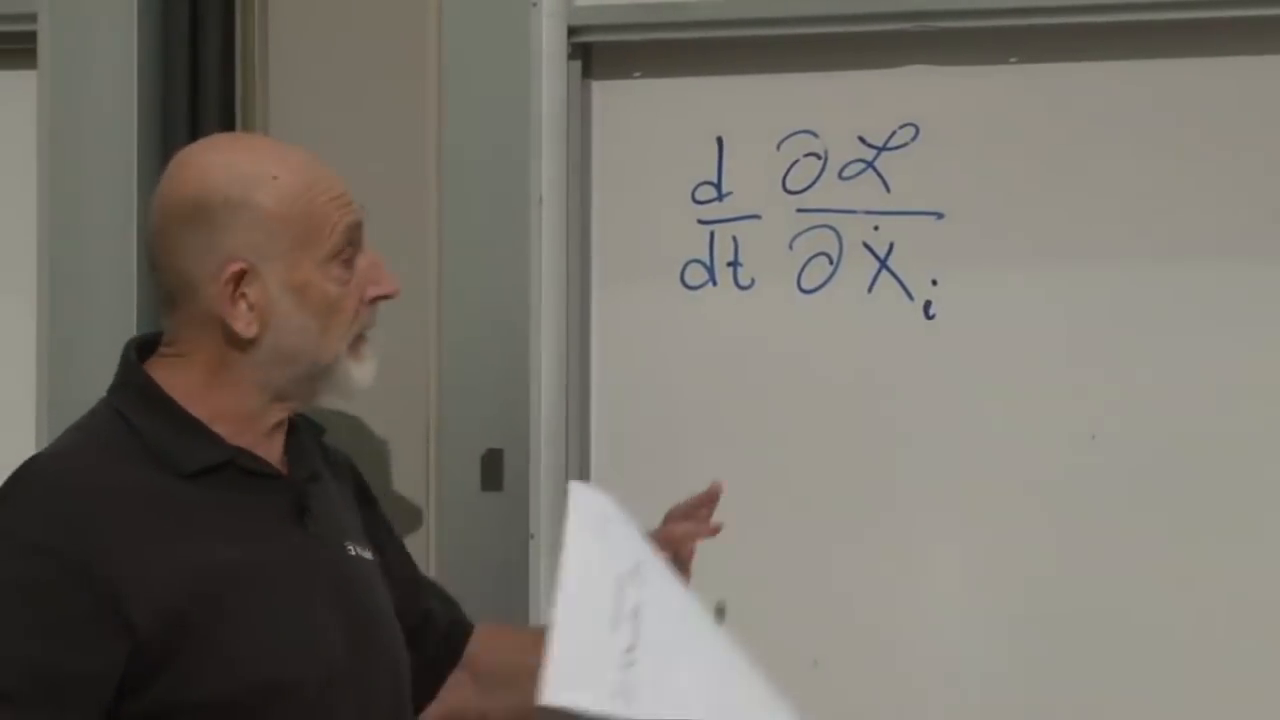
\includegraphics[width=0.76\textwidth]{lecture_04_figure_05.png}
  \caption{対称性と保存則の出発点として思い出されるEuler--Lagrange方程式。}
  \lectureframe{00:09:00}
\end{figure}

正しい表現は\emph{停留作用}であり、必ずしも最小作用ではない。この区別は終わりの近くで再び現れる。

\section{一般化座標と共役運動量}

Cartesian位置は一般力学にとって狭すぎる言語である。座標は粒子の位置、角度、集団変数、または場の振幅であり得るので、それらを\(q_i\)と呼ぶ。Lagrangianは力学の圧縮された指定である。非常に凝縮された記法なしに書き下されたStandard Modelでさえ、およそ1ページを占める。各場の成分に対して別々の運動方程式を書けば、はるかに多くの紙面を占めるであろう。一つの関数\(L\)がそれらすべてをまとめている。

\(q_i\)に共役な運動量は
\begin{equation}
  p_i=\frac{\partial L}{\partial\dot q_i}.
  \label{eq:canonical-momentum-l4}
\end{equation}
である。これが、一般化座標が伝統的に\(q\)の座標と呼ばれる理由である。対応する運動量は\(p\)の運動量であり、我々に\(p\)と\(q\)を与える。この記法では、式~\eqref{eq:el-l4}は
\begin{equation}
  \dot p_i=\frac{\partial L}{\partial q_i}.
  \label{eq:momentum-el-l4}
\end{equation}
になる。

おなじみの一次元粒子に対して、
\begin{equation}
  L=\frac{m\dot x^2}{2}-V(x),
  \qquad
  \frac{\partial L}{\partial\dot x}=m\dot x,
  \label{eq:particle-momentum-l4}
\end{equation}
なので、共役運動量は通常の運動量である。

\begin{figure}[htbp]
  \centering
  \includegraphics[width=0.72\textwidth]{lecture_04_figure_02.png}
  \caption{共役運動量を\(m\dot x\)と同定するために用いられる運動エネルギーからポテンシャルエネルギーを引いたLagrangian。}
  \lectureframe{00:14:48}
\end{figure}

\(q_i\)が\(L\)に現れないならば、\(\dot p_i=0\)である。これは保存則へのおなじみの循環座標の道筋である。本当のつながりはより一般的であり、証明する前に例でそれを見出すのが有用である。

\section{説明される前に見出された保存則}

\subsection{二つの座標と分離ポテンシャル}

両方の質量を1に等しく置き、
\begin{equation}
  L=\frac{\dot q_1^{\,2}+\dot q_2^{\,2}}{2}-V(q_1-q_2).
  \label{eq:separation-lagrangian}
\end{equation}
とする。直線上の二つの粒子を思い描いてもよい。それらの相互作用はそれらの分離のみに依存する。

\begin{figure}[htbp]
  \centering
  \includegraphics[width=0.78\textwidth]{lecture_04_figure_03.png}
  \caption{二座標のLagrangianとその第一運動量方程式の始まり。}
  \lectureframe{00:18:56}
\end{figure}

\(V\)の引数に関する微分を\(V'\)と書くと、
\begin{align}
  \dot p_1&=-V'(q_1-q_2),
  \notag\\
  \dot p_2&=+V'(q_1-q_2).
  \label{eq:separation-momentum-equations}
\end{align}
第二の符号が逆になるのは、\(q_2\)を増やすと\(q_1-q_2\)が減るからである。

\begin{classroomqa}
  \audiencequestion{第一の運動量方程式は\(V'\)を含むべきか、そしてそのマイナス符号はどこから来るのか。
  \lecturetimestamp{00:20:52--00:21:35}}
  \lecturerresponse{Euler--Lagrange方程式は
  \(\dot p_1=\partial L/\partial q_1\)と言っており、Lagrangianが零であるとは言っていない。
  \(L=T-V\)なので、\(q_1\)に関して微分すると
  \(-V'\)となる。\(q_2\)に関して微分すると\(q_1-q_2\)からもう一つマイナス符号が供給されるので、第二の方程式は\(+V'\)を持つ。}
\end{classroomqa}

\begin{figure}[htbp]
  \centering
  \includegraphics[width=0.78\textwidth]{lecture_04_figure_04.png}
  \caption{\(p_1\)方程式における符号に敏感な導関数。\(p_2\)方程式は反対の符号を受け取る。}
  \lectureframe{00:20:41}
\end{figure}

式~\eqref{eq:separation-momentum-equations}を加えると
\begin{equation}
  \frac{d}{dt}(p_1+p_2)=0.
  \label{eq:total-p-conserved}
\end{equation}
保存量を見出したが、それがなぜ存在するのかはまだ説明していない。

\subsection{あまり自明でない線形結合}

ここで
\begin{equation}
  L=\frac{\dot q_1^{\,2}+\dot q_2^{\,2}}{2}
    -V(Aq_1+Bq_2),
  \label{eq:ab-lagrangian}
\end{equation}
とおく。ただし\(A\)と\(B\)は定数である。すると
\begin{align}
  \dot p_1&=-A\,V'(Aq_1+Bq_2),
  \notag\\
  \dot p_2&=-B\,V'(Aq_1+Bq_2).
  \label{eq:ab-momentum-equations}
\end{align}
第一の方程式に\(B\)を掛け、第二の方程式に\(A\)を掛けて引き算すると、力が消去される：
\begin{equation}
  \frac{d}{dt}(Bp_1-Ap_2)=0.
  \label{eq:ab-conserved}
\end{equation}

\begin{figure}[htbp]
  \centering
  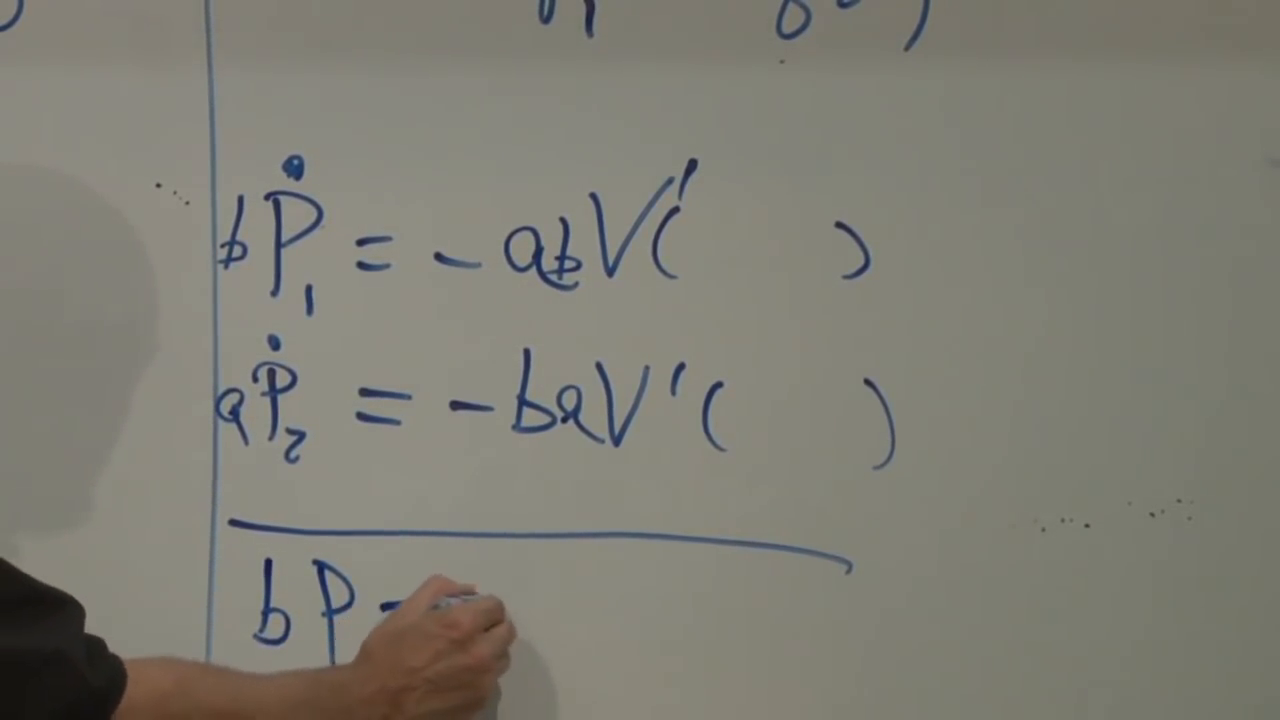
\includegraphics[width=0.78\textwidth]{lecture_04_figure_06.png}
  \caption{\(Bp_1-Ap_2\)において力の項が相殺する重み付き運動量方程式。}
  \lectureframe{00:24:20}
\end{figure}

\begin{classroomqa}
  \audiencequestion{\(A\)や\(B\)のような定数は物理的にどこから来るのだろうか。\lecturetimestamp{00:25:09--00:30:15}}
  \lecturerresponse{質量\(m\)と\(M\)の二つの粒子を考える：
  \[
    L=\frac{m\dot X^2}{2}+\frac{M\dot Y^2}{2}-V(X-Y).
  \]
  \(Q_1=\sqrt m\,X\)と\(Q_2=\sqrt M\,Y\)に再スケールする。運動項は
  \((\dot Q_1^2+\dot Q_2^2)/2\)となるが、ポテンシャルは
  \(Q_1/\sqrt m-Q_2/\sqrt M\)に依存する。したがって、等しくない質量は自然に線形結合の係数となる。\(Q_2\)を\(-Q_2\)に置き換えると、表示されているマイナスがプラスに変わるが、その二乗された運動項は変わらない。}
\end{classroomqa}

\begin{figure}[htbp]
  \centering
  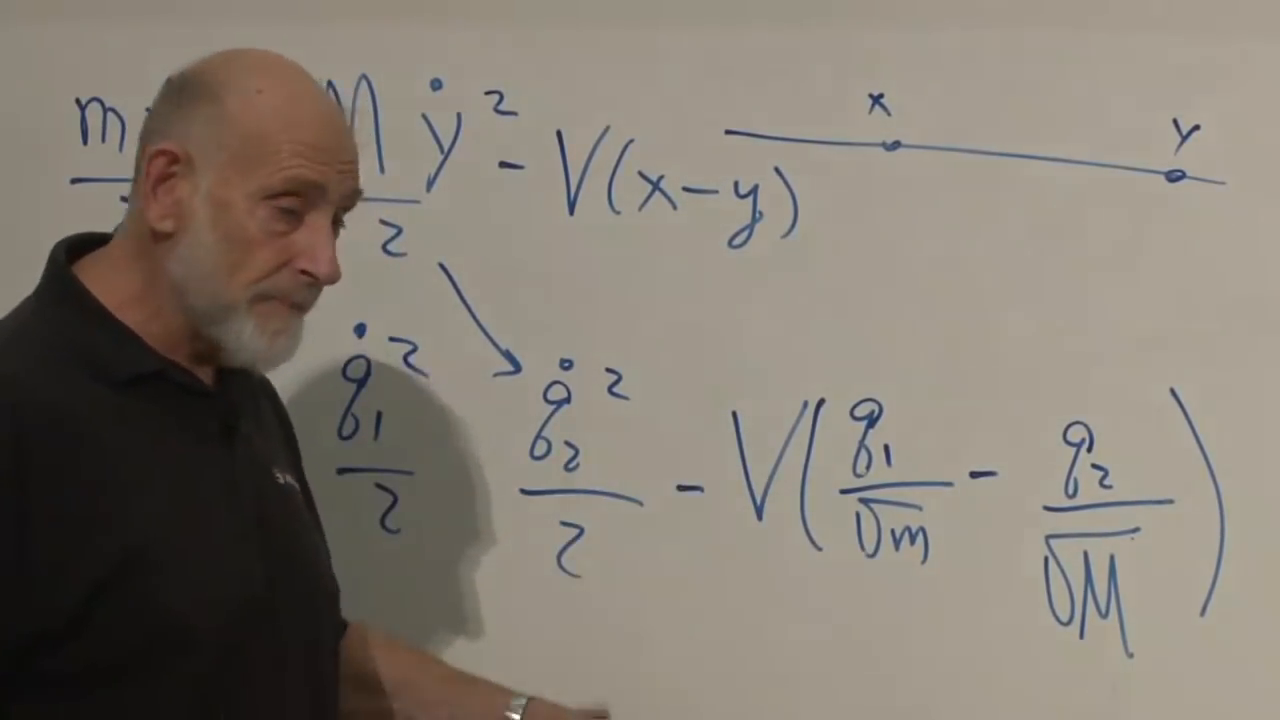
\includegraphics[width=0.82\textwidth]{lecture_04_figure_07.png}
  \caption{質量で重み付けした座標は運動エネルギーを簡単にする一方で、質量因子をポテンシャルへ移す。}
  \lectureframe{00:28:40}
\end{figure}

\begin{classroomqa}
  \audiencequestion{これは、循環座標がなくても保存量が存在しうることを示しているのか。\lecturetimestamp{00:31:13--00:31:58}}
  \lecturerresponse{書かれている変数のままでは、\emph{明白な}循環座標は存在しない。変数を変えればそれが現れるかもしれないが、それを探すことはここでの有用な視点ではない。対称性の議論が保存される組み合わせを直接同定するであろう。}
\end{classroomqa}

\section{対称性とは何を意味するか}

\subsection{並進}

単位質量の自由粒子から始める：
\begin{equation}
  L=\frac{\dot q^2}{2}.
  \label{eq:free-unit-l4}
\end{equation}
その履歴のすべての点を同じ定数だけ並進させる：
\begin{equation}
  q'(t)=q(t)+\epsilon.
  \label{eq:free-translation}
\end{equation}
\(\epsilon\)は時間に依存しないので、\(\dot q'=\dot q\)であり、したがって
\(\delta L=0\)。この不変性が並進対称性である。

二つの等価な描像がある。受動的には、物体を固定したまま座標原点をずらす。能動的には、軸を固定したまま物体を動かす。能動的な言葉遣いのほうが混乱が少ないことがわかるであろう。物理的配置を動かし、\(L\)が気づくかどうかを問うのである。

式~\eqref{eq:separation-lagrangian}について、両方の座標を並進させる：
\begin{equation}
  \delta q_1=\epsilon,
  \qquad
  \delta q_2=\epsilon.
  \label{eq:common-translation}
\end{equation}
速度は変わらず、\(q_1-q_2\)も変わらない。

\begin{figure}[htbp]
  \centering
  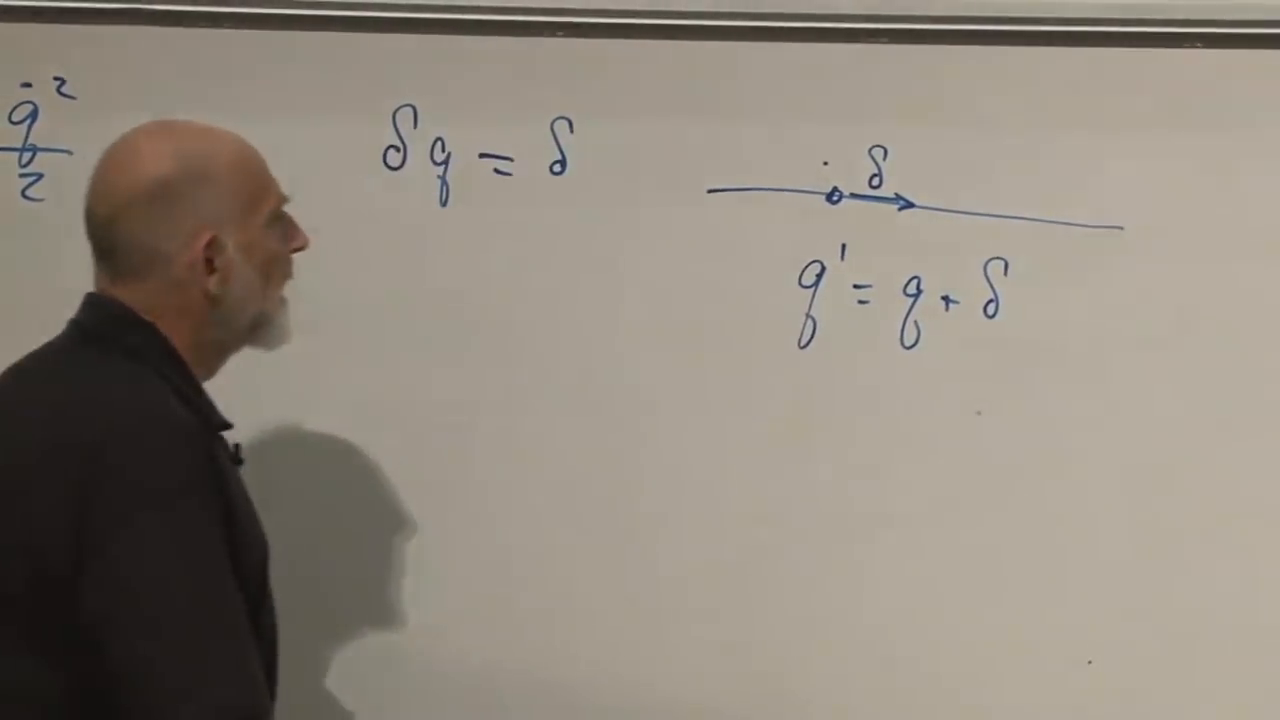
\includegraphics[width=0.78\textwidth]{lecture_04_figure_08.png}
  \caption{共通の並進は二つの座標の差を変えない。}
  \lectureframe{00:35:30}
\end{figure}

式~\eqref{eq:ab-lagrangian}について、あまり自明でない変換を用いる：
\begin{equation}
  \delta q_1=B\epsilon,
  \qquad
  \delta q_2=-A\epsilon.
  \label{eq:ab-transformation}
\end{equation}
ここでも速度は変わらないが、
\begin{equation}
  \delta(Aq_1+Bq_2)=AB\epsilon-BA\epsilon=0.
  \label{eq:ab-invariant-argument}
\end{equation}
したがってこの変換は対称性である。

\begin{figure}[htbp]
  \centering
  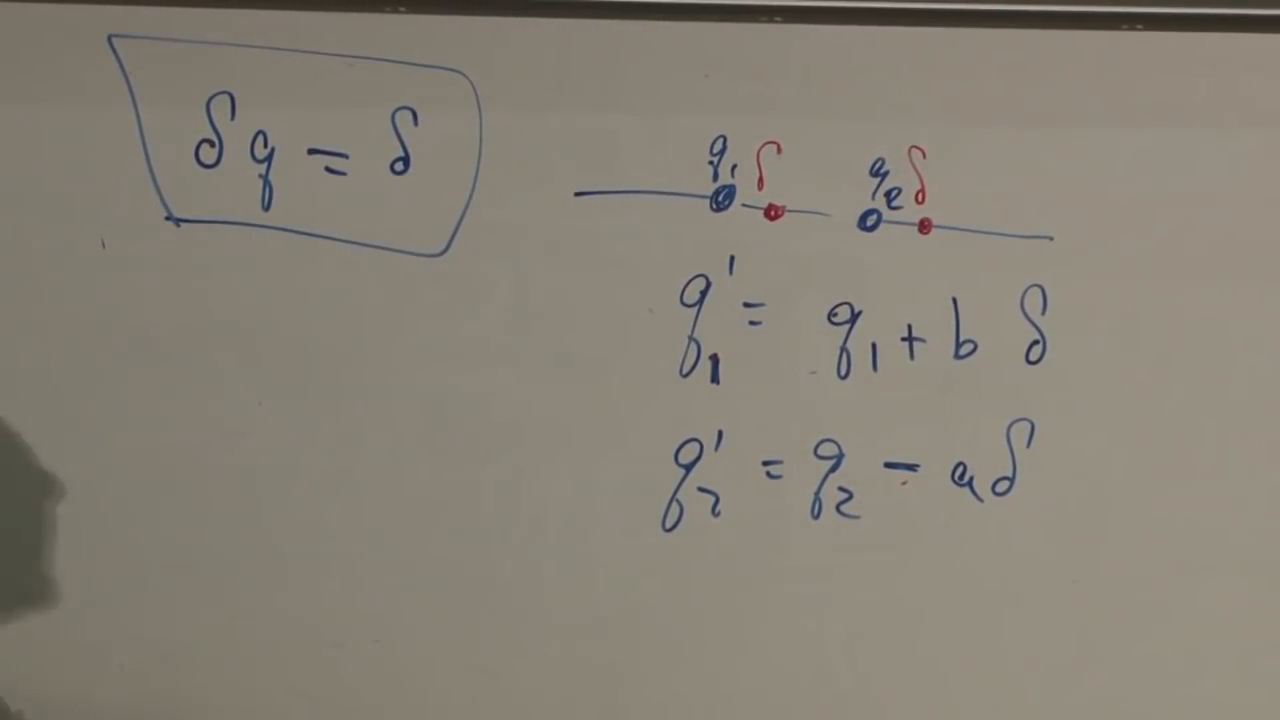
\includegraphics[width=0.80\textwidth]{lecture_04_figure_09.png}
  \caption{\(Aq_1+Bq_2\)を保つ非対称な並進。}
  \lectureframe{00:40:20}
\end{figure}

\begin{classroomqa}
  \audiencequestion{係数は質量を符号化しており、保存量は通常の重心運動量になるのか。
  \lecturetimestamp{00:42:25--00:42:45}}
  \lecturerresponse{はい。質量で重み付けした変数では、対称性と保存される組み合わせは非対称に見える。\(X\)と\(Y\)に戻すと、通常の同時並進と全運動量が回復される。}
\end{classroomqa}

\subsection{回転}

平面上の一粒子を考える：
\begin{equation}
  L=\frac{m}{2}(\dot x^2+\dot y^2)-V(x^2+y^2).
  \label{eq:central-lagrangian-l4}
\end{equation}
これは中心ポテンシャルである。互いに回転した二つの固定座標系を比較する。軸は時間的に回転していない。一つの整合した向きのもとで、
\begin{align}
  x'&=x\cos\theta+y\sin\theta,
  \notag\\
  y'&=-x\sin\theta+y\cos\theta.
  \label{eq:finite-rotation-l4}
\end{align}

\begin{figure}[htbp]
  \centering
  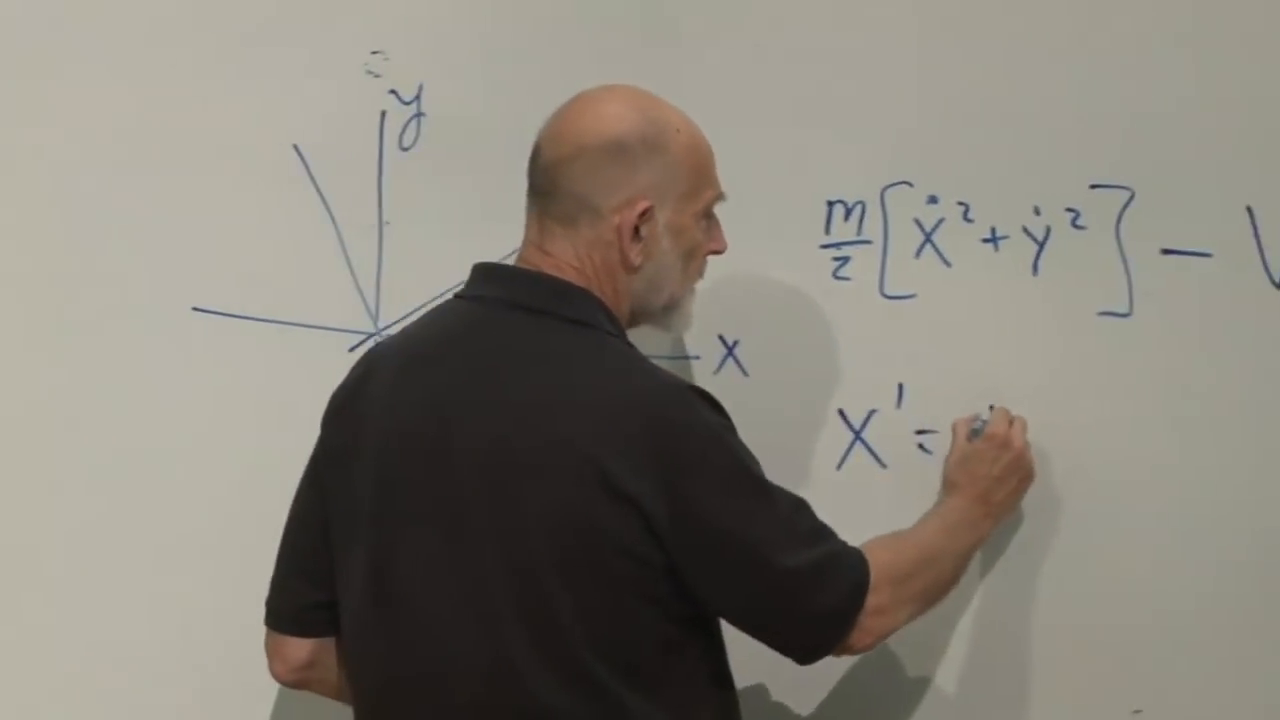
\includegraphics[width=0.82\textwidth]{lecture_04_figure_10.png}
  \caption{中心ポテンシャルのラグランジアンと、回転で関係づけられた二つの固定デカルト座標系。}
  \lectureframe{00:45:40}
\end{figure}

\(\theta=\epsilon\)とおき、一次まで保つ：
\begin{equation}
  \cos\epsilon=1+O(\epsilon^2),
  \qquad
  \sin\epsilon=\epsilon+O(\epsilon^3).
  \label{eq:small-angle-l4}
\end{equation}
無限小回転は
\begin{align}
  \delta x&=y\epsilon,
  &\delta y&=-x\epsilon,
  \notag\\
  \delta\dot x&=\dot y\epsilon,
  &\delta\dot y&=-\dot x\epsilon.
  \label{eq:infinitesimal-rotation-l4}
\end{align}

\begin{figure}[htbp]
  \centering
  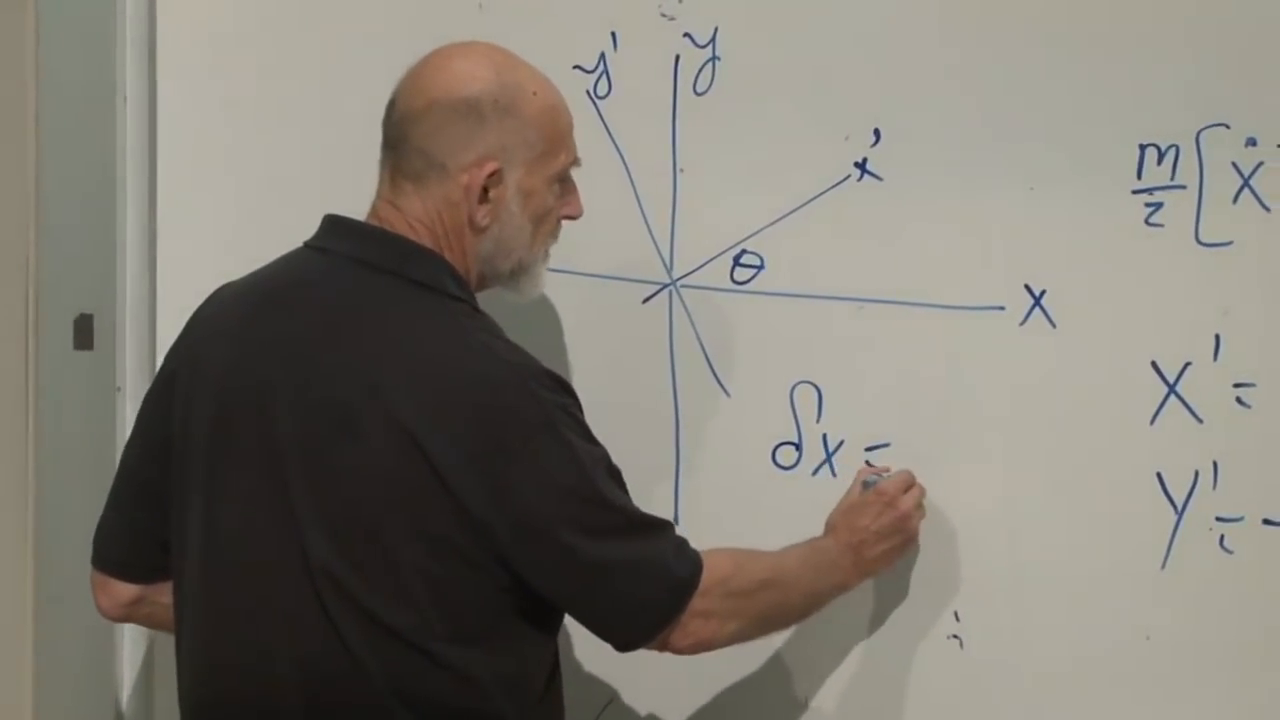
\includegraphics[width=0.82\textwidth]{lecture_04_figure_11.png}
  \caption{座標と速度の無限小回転。}
  \lectureframe{00:49:50}
\end{figure}

並進とは異なり、\(x\)が変化する量は\(y\)に依存し、\(y\)が変化する量は\(x\)に依存する。それにもかかわらず、
\begin{align}
  \delta(x^2+y^2)
  &=2x\,\delta x+2y\,\delta y=0,
  \notag\\
  \delta(\dot x^2+\dot y^2)
  &=2\dot x\,\delta\dot x+2\dot y\,\delta\dot y=0.
  \label{eq:rotation-invariants-l4}
\end{align}
ポテンシャル項も運動項も不変である。

\begin{figure}[htbp]
  \centering
  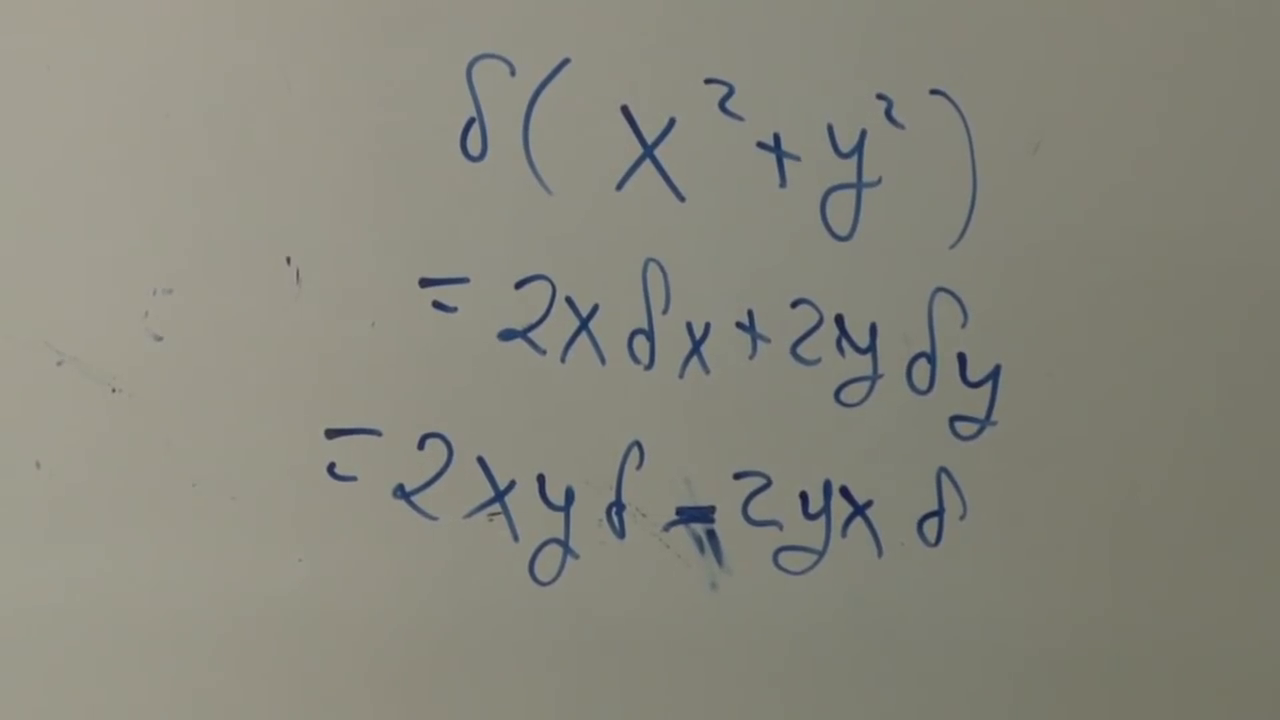
\includegraphics[width=0.76\textwidth]{lecture_04_figure_12.png}
  \caption{二乗半径が回転不変であることを証明する一次の相殺。}
  \lectureframe{00:53:20}
\end{figure}

\section{一般的な保存定理}

並進と回転の例には共通する一つの形がある。連続的な無限小変換を
\begin{equation}
  \delta q_i=\epsilon f_i(q),
  \qquad
  \delta\dot q_i=\frac{d}{dt}\delta q_i,
  \label{eq:general-infinitesimal-symmetry}
\end{equation}
とする。ただし\(\epsilon\)は時間に依存せず、\(f_i\)はすべての座標に依存しうる。

\begin{figure}[htbp]
  \centering
  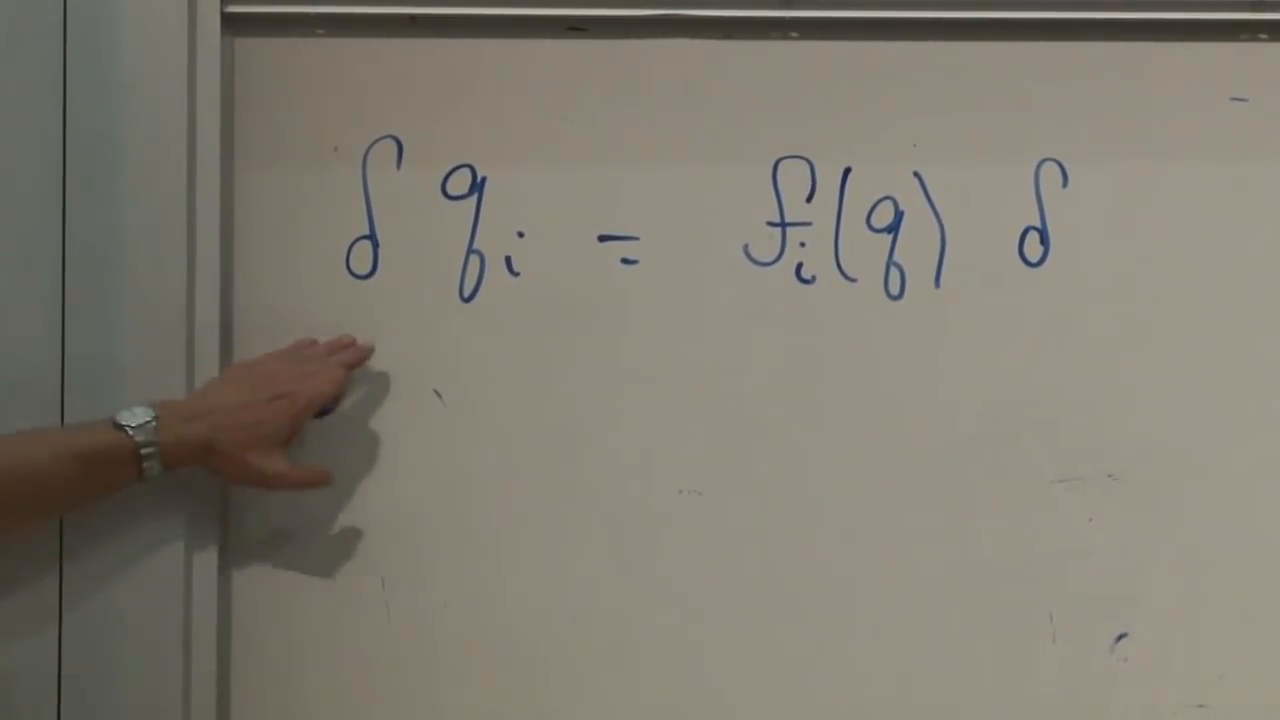
\includegraphics[width=0.78\textwidth]{lecture_04_figure_13.png}
  \caption{一般的な無限小変位場
  \(\delta q_i=\epsilon f_i(q)\)。}
  \lectureframe{00:56:00}
\end{figure}

ラグランジアンの一次変分は
\begin{equation}
  \delta L
  =\sum_i\left(
    \frac{\partial L}{\partial q_i}\delta q_i
    +\frac{\partial L}{\partial\dot q_i}\delta\dot q_i
  \right).
  \label{eq:delta-l-general}
\end{equation}

\begin{figure}[htbp]
  \centering
  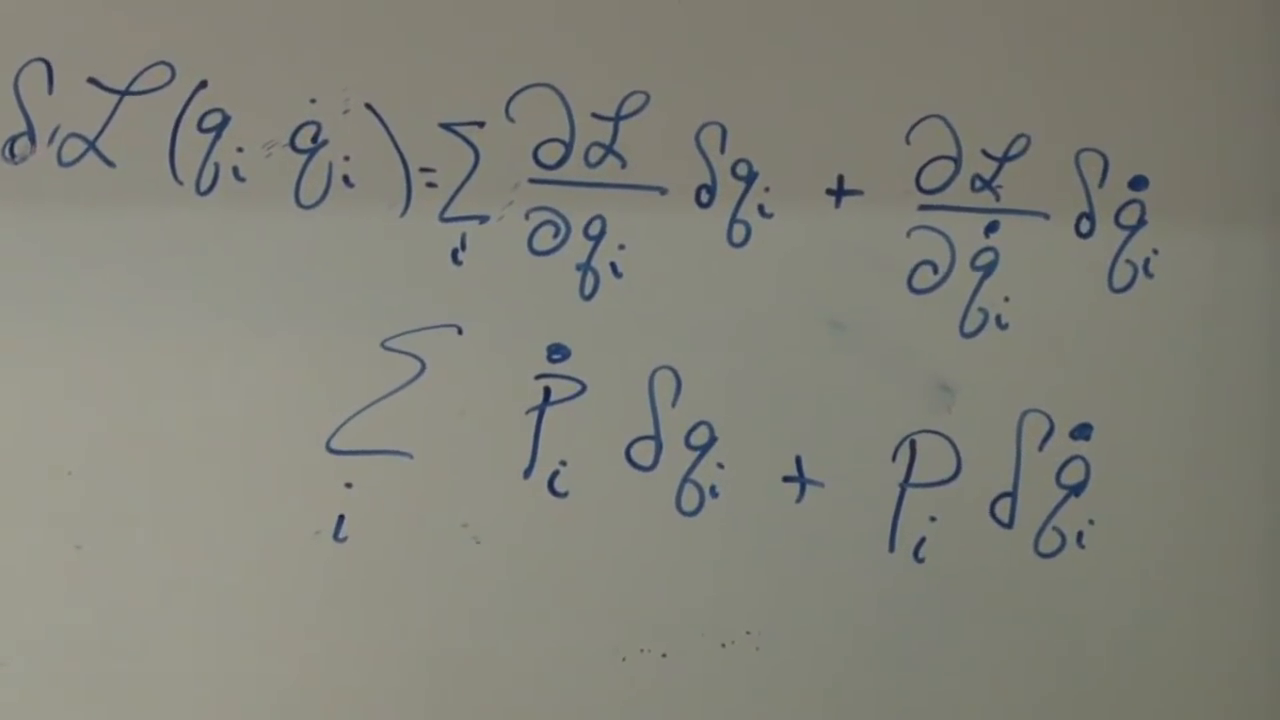
\includegraphics[width=0.84\textwidth]{lecture_04_figure_14.png}
  \caption{\(\delta L\)への二つの寄与：座標の変分と
  速度の変分。}
  \lectureframe{01:02:30}
\end{figure}

ここで物理的な経路に注目を限定すると、Euler--Lagrange方程式が
成り立つ。
\begin{equation}
  \frac{\partial L}{\partial\dot q_i}=p_i,
  \qquad
  \frac{\partial L}{\partial q_i}=\dot p_i,
  \label{eq:el-substitution-l4}
\end{equation}
を用いると
\begin{align}
  \delta L
  &=\sum_i\left(\dot p_i\,\delta q_i
                +p_i\,\delta\dot q_i\right)
  \notag\\
  &=\frac{d}{dt}\sum_i p_i\delta q_i
  =\epsilon\frac{d}{dt}\sum_i p_i f_i(q).
  \label{eq:noether-derivation-l4}
\end{align}
が得られる。中心となる手順は積の微分則のみである。

変換が対称性ならば、\(\delta L=0\)。\(\epsilon\) は
任意の定数因子であるから、
\begin{equation}
  \boxed{
  \frac{d\mathcal Q}{dt}=0,
  \qquad
  \mathcal Q=\sum_i p_i f_i(q)}
  .
  \label{eq:noether-charge-l4}
\end{equation}
これが、厳密で時間に依存しない点対称性に対するNoetherの定理の古典力学における中核である。

\begin{figure}[htbp]
  \centering
  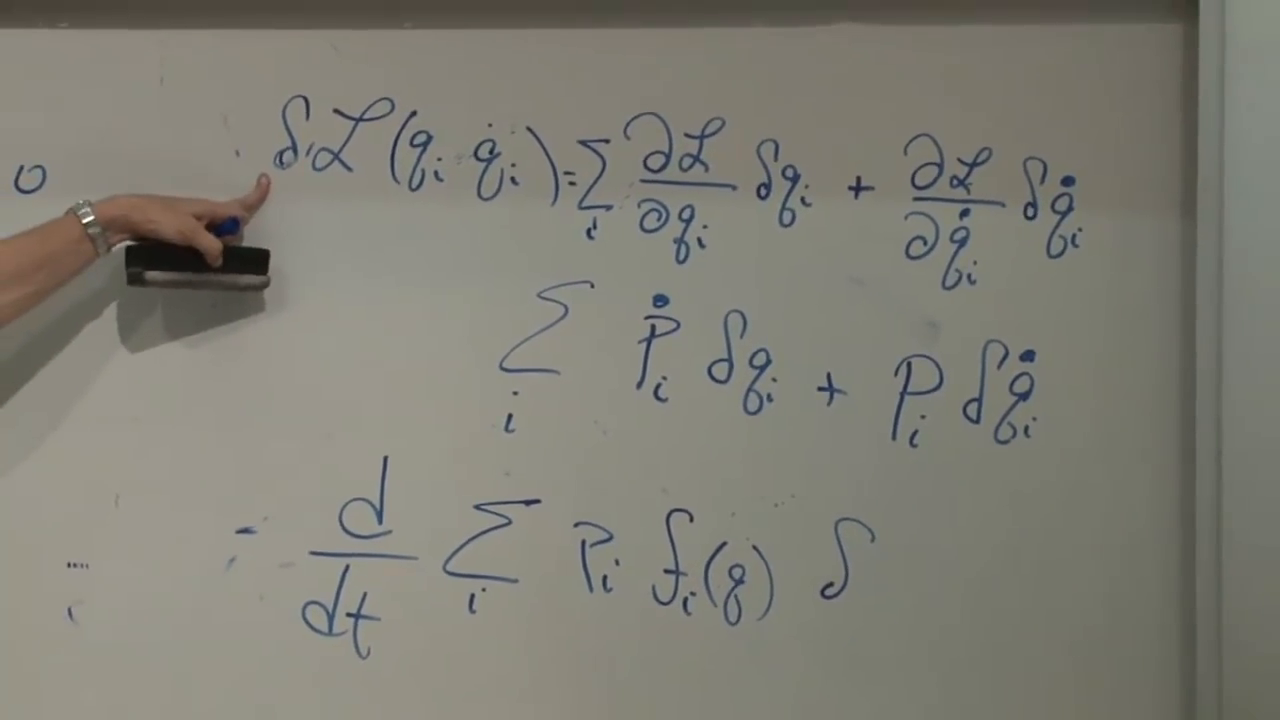
\includegraphics[width=0.84\textwidth]{lecture_04_figure_15.png}
  \caption{\(L\)の不変性を保存量に変える
  積の微分則の手順。}
  \lectureframe{01:05:00}
\end{figure}

\begin{classroomqa}
  \audiencequestion{\(f_i(q)\)において、\(q\)は別の添字を持つか？
  \lecturetimestamp{01:06:57--01:07:31}}
  \lecturerresponse{添字のない\(q\)は集合全体
  \((q_1,q_2,\ldots)\)を表す。各成分\(f_i\)はそれらすべての
  座標に依存しうる。例えば回転では、\(f_x=y\)および\(f_y=-x\)である。}
\end{classroomqa}

これらの例はもはや偶然ではない。共通の並進では
\(f_1=f_2=1\)、したがって
\begin{equation}
  \mathcal Q=p_1+p_2.
  \label{eq:noether-common-p}
\end{equation}
非対称な並進では\(f_1=B\)、\(f_2=-A\)、したがって
\begin{equation}
  \mathcal Q=Bp_1-Ap_2.
  \label{eq:noether-ab-p}
\end{equation}
回転では\(f_x=y\)および\(f_y=-x\)：
\begin{equation}
  \mathcal Q=p_xy-p_yx.
  \label{eq:rotation-charge-sign}
\end{equation}
向きの符号を除けば、これは角運動量
\begin{equation}
  J=xp_y-yp_x.
  \label{eq:angular-momentum-l4}
\end{equation}である。

\begin{figure}[htbp]
  \centering
  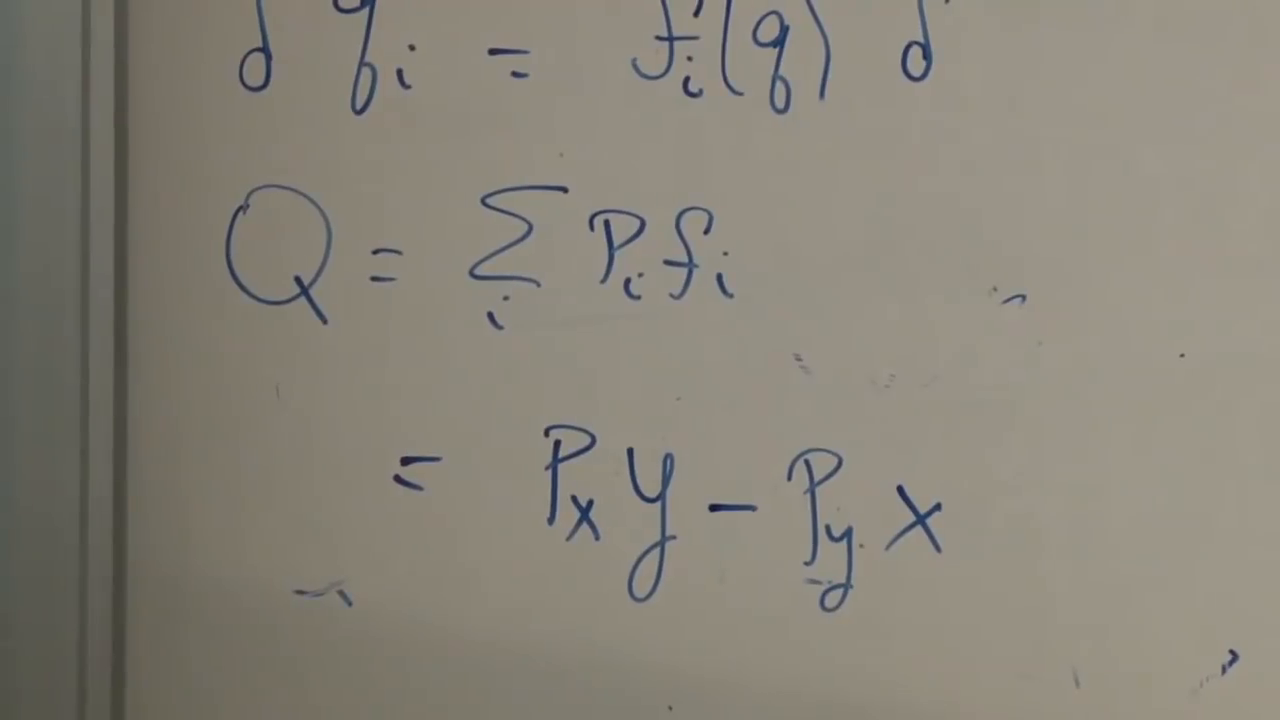
\includegraphics[width=0.82\textwidth]{lecture_04_figure_16.png}
  \caption{回転のNoether電荷。向きを除いて平面内の
  角運動量に等しい。}
  \lectureframe{01:11:00}
\end{figure}

多数の相互作用する粒子に対しては、すべての粒子を一緒に回転させる。そのとき不変性はそれらの角運動量の和を保存し、各粒子の角運動量を別々に保存するのではない。

\section{定理の仮定に関する質問}

\begin{classroomqa}
  \audiencequestion{回転する座標軸の組は\(\delta L\)に明示的な時間依存性を導入するか？\lecturetimestamp{01:12:57--01:13:57}}
  \lecturerresponse{はい。今行った証明は時間に依存しない
  対称性パラメータ、すなわち固定された並進または固定された回転を仮定している。
  パラメータが時間に依存する変換は付加的な項を生じ、
  より一般的な取り扱いを必要とする。}
\end{classroomqa}

\begin{classroomqa}
  \audiencequestion{黒板の式の大文字の\(Q\)は
  変換そのものか？\lecturetimestamp{01:14:02--01:15:58}}
  \lecturerresponse{いいえ。その記法は残念ながら
  座標\(q_i\)と衝突する。変換は
  \(\delta q_i=\epsilon f_i(q)\)であり、結果として得られる保存量は
  \(\mathcal Q=\sum_i p_i f_i\)である。係数\(f_i\)は
  \(i\)番目の座標が対称性の下でどのように動くかを示す。}
\end{classroomqa}

エネルギー保存もまた対称性によって生成されるが、それは別の対称性である：時間並進、すなわち時間の零点をどこに置くかに依存しないことである。その場合とHamilton形式については後回しにする。

\begin{classroomqa}
  \audiencequestion{実際の運動を変化する座標系に吸収し、力学を
  単なる座標変換にすることはできるか？\lecturetimestamp{01:17:43--01:20:01}}
  \lecturerresponse{特定の運動に追随する座標を選ぶことはできるが、
  そのとき変換は初期状態と軌道に依存する。ここで用いた対称性変換は、
  系がどの解に従うかとは独立に固定されている。運動そのものは
  座標と運動量の合成空間においてより自然に表される。}
\end{classroomqa}

\section{位相空間における調和振動子}

質量とばね定数を1に設定すると、
\begin{equation}
  L=\frac{\dot q^2}{2}-\frac{q^2}{2}.
  \label{eq:oscillator-l4}
\end{equation}
共役運動量と運動方程式から
\begin{equation}
  p=\dot q,
  \qquad
  \dot p=-q,
  \label{eq:oscillator-first-order-l4}
\end{equation}
または
\begin{equation}
  \dot q=p,
  \qquad
  \dot p=-q.
  \label{eq:oscillator-phase-flow}
\end{equation}
これらの方程式は\(q\)-\(p\)平面における等速円運動を記述する。
実空間で往復する振動子はその円の\(q\)軸への射影である：速さは\(q=0\)で最大となり、
転回点で消える。

\begin{figure}[htbp]
  \centering
  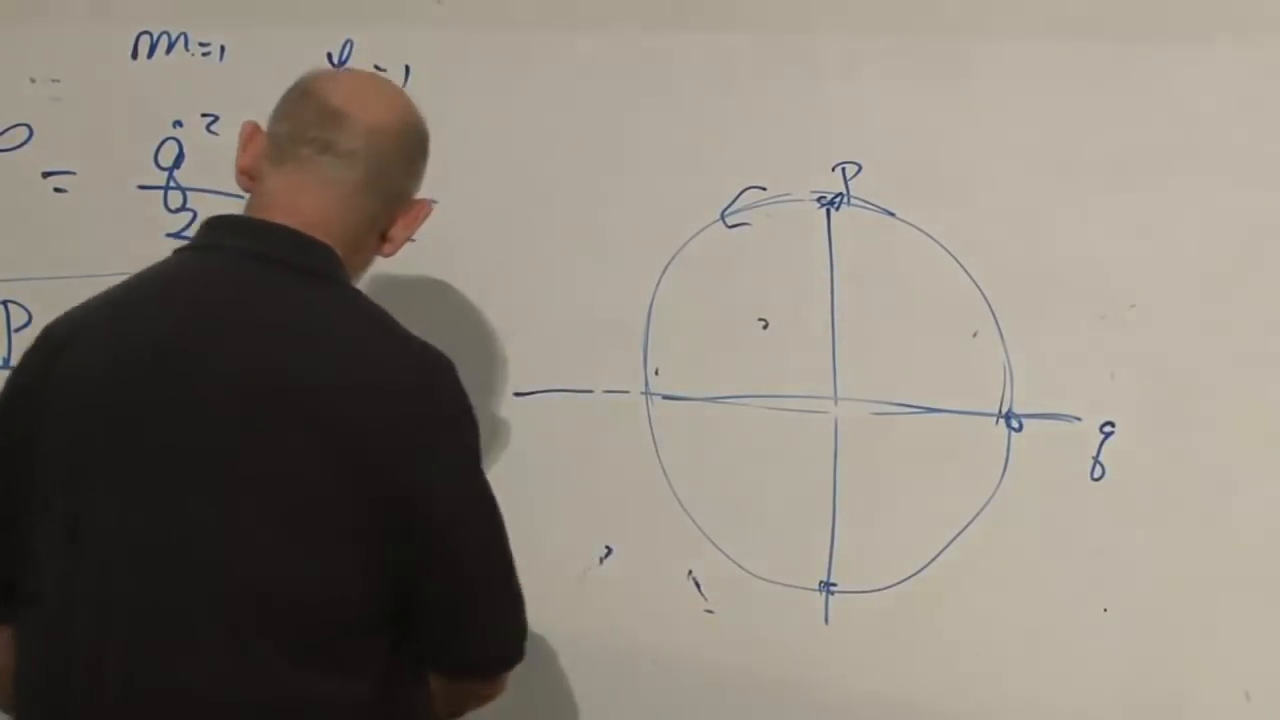
\includegraphics[width=0.82\textwidth]{lecture_04_figure_17.png}
  \caption{調和振動子の方程式と\(q\)-\(p\)空間における
  その円軌道。}
  \lectureframe{01:25:30}
\end{figure}

\begin{classroomqa}
  \audiencequestion{位相空間の円は時計回りに回るか？
  \lecturetimestamp{01:25:47--01:27:15}}
  \lecturerresponse{\(p\)を水平に、\(q\)を垂直にとると、はい。
  正の最大の\(q\)では\(\dot p=-q<0\)なので、運動は下向きである。
  軸の配置を逆にすると見かけの向きが逆になり、
  それゆえこの規約は誤って覚えやすい。}
\end{classroomqa}

式~\eqref{eq:oscillator-phase-flow}の組はすでにHamiltonの方程式に似ているが、それは完全にLagrange力学の枠内で得られたものである。

\section{連続対称性と離散対称性}

\begin{classroomqa}
  \audiencequestion{対称性は無限小のデカルト変換によって表されなければならないのだろうか。\lecturetimestamp{01:27:48--01:30:31}}
  \lecturerresponse{デカルト座標は便利なだけであり、この証明に本質的に必要なのは連続性である。ある種の対称性には無限小版が存在しない。偶ポテンシャルに対して、鏡映は\(q\mapsto -q\)および\(\dot q\mapsto-\dot q\)を送り、\(L\)を不変に保つが、鏡映を任意に小さな鏡映から組み立てることはできない。したがってこの古典的導出からは、対応する保存量は得られない。}
\end{classroomqa}

\begin{figure}[htbp]
  \centering
  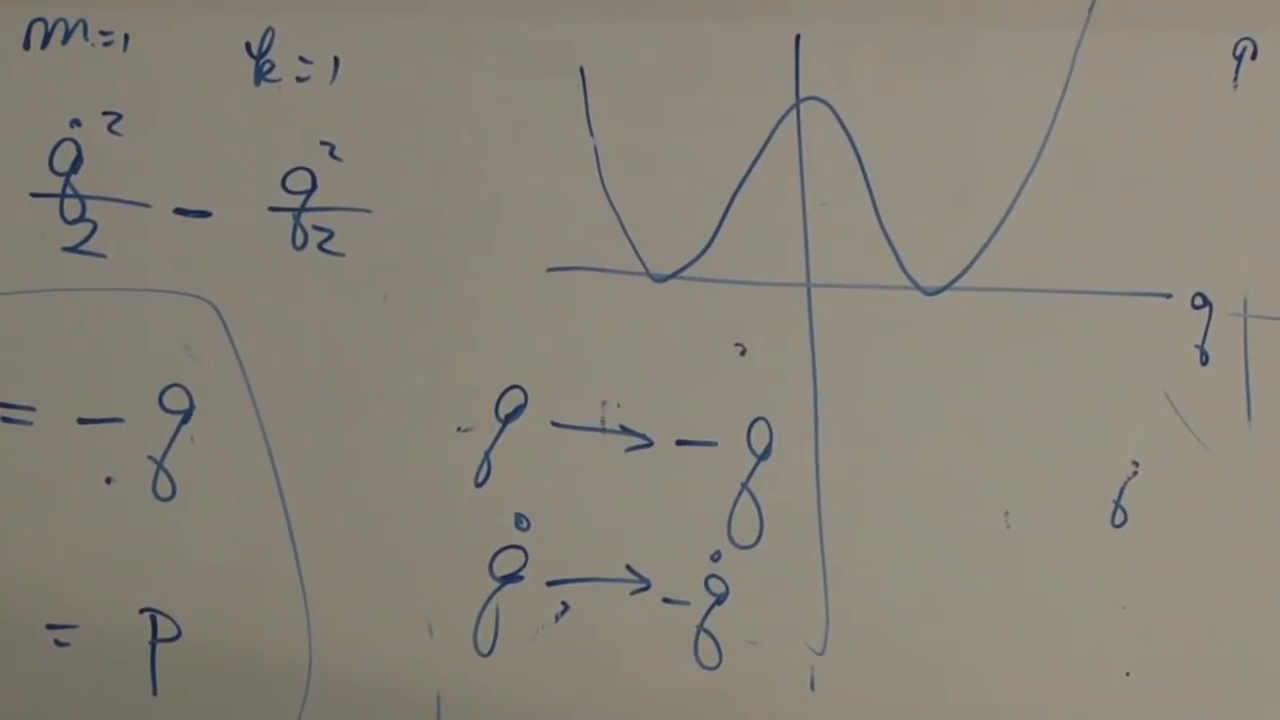
\includegraphics[width=0.82\textwidth]{lecture_04_figure_18.png}
  \caption{偶ポテンシャルは離散鏡映\(q\mapsto -q\)の下で不変である。}
  \lectureframe{01:29:30}
\end{figure}

\begin{classroomqa}
  \audiencequestion{保存量\(\mathcal Q\)が非零であるならば、それは変換が対称性ではなかったことを示すのだろうか。
  \lecturetimestamp{01:30:40--01:31:30}}
  \lecturerresponse{いいえ。保存量は任意の一定値をとりうる。関係する判定基準は\(\dot{\mathcal Q}\)である。提案された変換から導かれる量が保存されないならば、その提案された変換はこの証明の仮定の下では対称性ではなかったのである。}
\end{classroomqa}

\begin{classroomqa}
  \audiencequestion{鏡映は依然としてラグランジアンを不変に保つのに、なぜそれから保存則が得られないのか。\lecturetimestamp{01:31:34--01:32:27}}
  \lecturerresponse{不変性それ自体は見て取れるが、導出は一次の変位と積の法則を経由した。鏡映は配置空間の一方の側を一回の離散的なステップで他方の側へ移す。無限小生成子\(f_i\)がなければ、式\(\mathcal Q=\sum_i p_i f_i\)には使うものがない。}
\end{classroomqa}

\begin{classroomqa}
  \audiencequestion{任意に小さな変換から組み立てられるという性質の名前は何か。\lecturetimestamp{01:32:36--01:33:23}}
  \lecturerresponse{それは\emph{連続対称性}である。並進と回転は連続であり、鏡映は\emph{離散対称性}である。}
\end{classroomqa}

\begin{classroomqa}
  \audiencequestion{多くの無限小ステップが有限変換を作るならば、捨てられた\(O(\epsilon^2)\)の誤差は蓄積しうるのだろうか。
  \lecturetimestamp{01:33:23--01:36:10}}
  \lecturerresponse{無限小の不変性は、出発点だけでなく、変換に沿って到達する各点で成り立たなければならない。有限のパラメータ区間を大きさ\(\epsilon\)の\(N\)個のステップに分割すると、蓄積された一次の変位は\(N\epsilon\)であり、一方、局所的な\(O(\epsilon^2)\)の剰余は\(N\epsilon^2=(N\epsilon)\epsilon\to0\)として蓄積する。これが連続変換群によって形式化される局所から有限への構造である。}
\end{classroomqa}

\begin{classroomqa}
  \audiencequestion{離散対称性は古典系において物理的に実現されているのだろうか。\lecturetimestamp{01:36:32--01:37:25}}
  \lecturerresponse{もちろんである。調和振動子それ自体が偶ポテンシャル\(V(q)\propto q^2\)をもつので、\(q\mapsto -q\)の下で不変である。そのような例は数多くある。要点はただ、この離散的不変性が新たな古典的ネーター電荷を与えないということだけである。}
\end{classroomqa}

\begin{classroomqa}
  \audiencequestion{しかし、連続変換と離散変換の両方が\(L\)を不変に保つならば、それは同じ条件ではないのか。
  \lecturetimestamp{01:37:37--01:39:18}}
  \lecturerresponse{それは不変性の同じ有限的な言明ではあるが、この証明への同じ数学的入力ではない。証明には一次の変分が必要である。鏡映に対しては「一次」ということが意味をもたないので、電荷に至る方程式の連鎖はそもそも始めることさえできない。}
\end{classroomqa}

\begin{classroomqa}
  \audiencequestion{これは歴史的にネーターの定理とどのように関係するのか。
  \lecturetimestamp{01:39:26--01:40:42}}
  \lecturerresponse{これはエミー・ネーターのはるかに一般的な定理の制限された一部分である。対称性と保存量の間の個々の関連は以前から知られていたが、ネーターはそれらを二十世紀初頭に統一され、驚くほど一般的な枠組みに置いた。彼女の数学的重要性は、公正な学術的扱いによって報われることはなかった。}
\end{classroomqa}

\begin{classroomqa}
  \audiencequestion{古典力学は今なお活発な研究主題なのだろうか。\lecturetimestamp{01:40:47--01:42:37}}
  \lecturerresponse{はい。ここで用いられた初等的な定理は古いが、非線形力学、可積分系、カオス、流体、幾何学的力学は依然として豊かな主題である。対称性の原理もまた、古典的粒子力学をはるかに超えて続いている。}
\end{classroomqa}

\section{なぜ作用原理が重要か}

\begin{classroomqa}
  \audiencequestion{対称性が保存則を意味するはずだという直観的な理由はありますか。\lecturetimestamp{01:42:49--01:47:57}}
  \lecturerresponse{対称性だけからではありません。粘性抵抗を考えます。
  \[
    m\ddot x=-c\dot x.
  \]
  この方程式は\(x\mapsto x+\epsilon\)の下で不変ですが、
  \(p=m\dot x\)として、
  \[
    \dot p=-\frac{c}{m}p,
    \qquad
    p(t)=p(0)e^{-ct/m},
  \]
  したがって運動量は減衰します。これは部分系に対する有効方程式であり、\(x\)だけに対する基本的な停留作用の法則ではありません。流体分子と閉じた系の残りを含めれば、全運動量は保存されます。対称性と保存則は、微分方程式の見かけだけによってではなく、ラグランジアン作用原理を通じて結びついています。}
\end{classroomqa}

\begin{figure}[htbp]
  \centering
  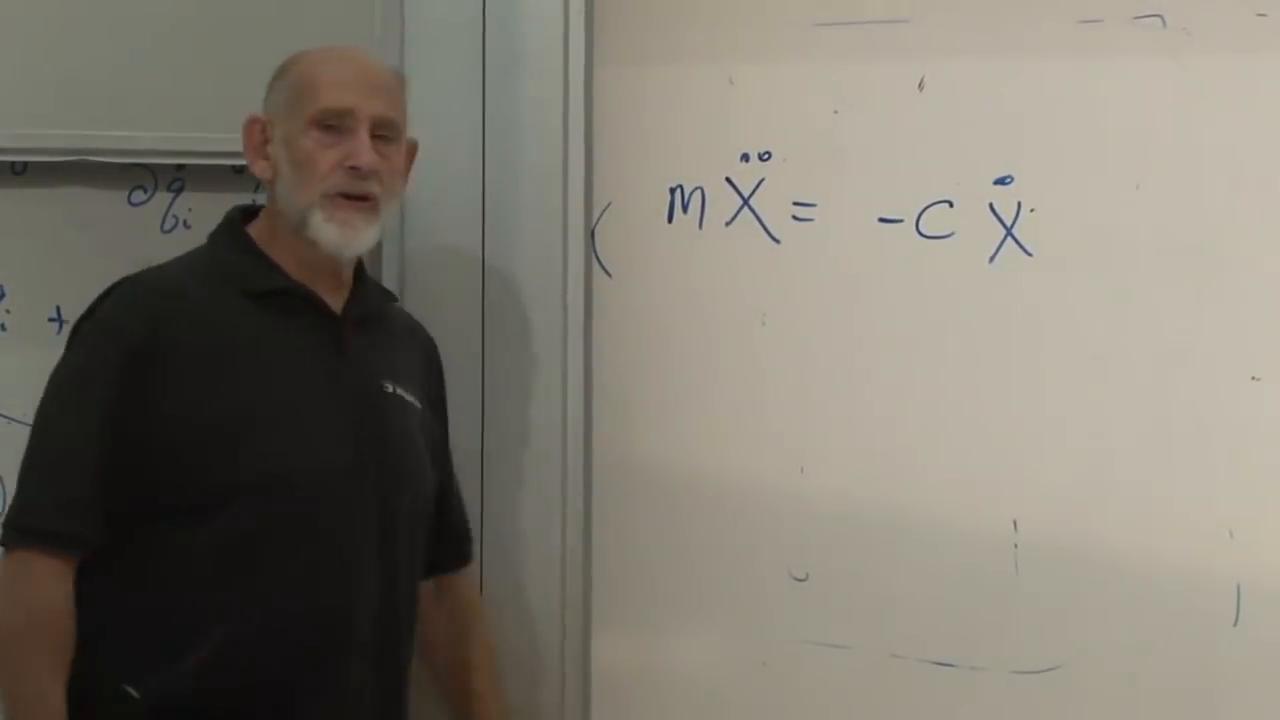
\includegraphics[width=0.65\textwidth]{lecture_04_figure_19.png}
  \caption{並進不変な粘性抵抗。しかしその換算された粒子運動量は減衰する。}
  \lectureframe{01:44:30}
\end{figure}

\begin{classroomqa}
  \audiencequestion{物理的な経路が作用の最小値でないのはどのような場合か、定量化できますか。\lecturetimestamp{01:48:08--01:51:38}}
  \lecturerresponse{真の最小値は例外的であり、作用は一般に経路空間における鞍点です。単位振動子では、
  \[
    S[q]=\frac12\int(\dot q^2-q^2)\,dt.
  \]
  狭く急速に変化する変形は正の\(\dot q^2\)の寄与を増大させます。長い時間わずかに変位したままとどまる広い変形は、負の\(-q^2\)の寄与を支配的にし、作用を低下させ得ます。したがって同じ停留経路が増加する方向と減少する方向をもちます。量子力学は経路積分の観点を通じて、停留性のより深い起源を与えますが、その議論は後回しにします。}
\end{classroomqa}

\begin{figure}[htbp]
  \centering
  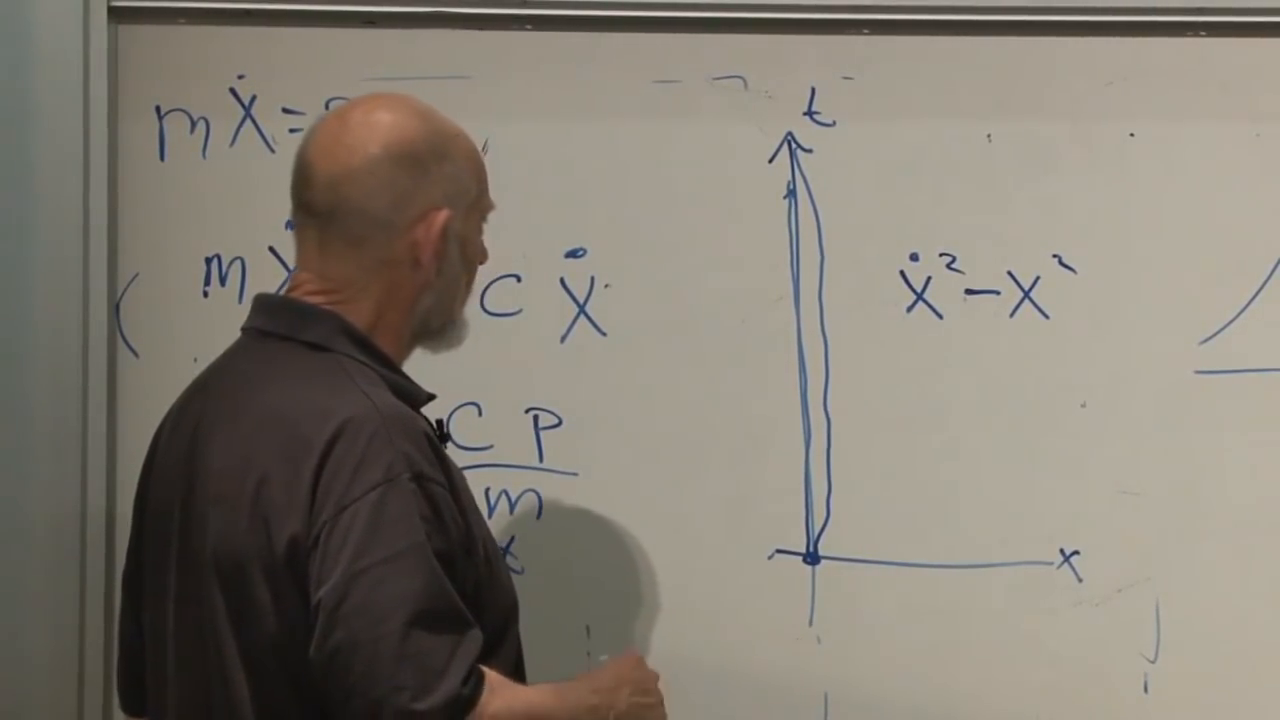
\includegraphics[width=0.80\textwidth]{lecture_04_figure_20.png}
  \caption{広い隣接振動子経路は、停留作用が典型的には最小値ではなく鞍点である理由を例示する。}
  \lectureframe{01:50:20}
\end{figure}

\begin{classroomqa}
  \audiencequestion{連続対称性と保存則の間には一対一の対応がありますか。\lecturetimestamp{01:51:44--01:52:43}}
  \lecturerresponse{変分設定の範囲内で、等価な場合や自明な場合を同一視した後では、本質的にその描像は正しいです。すべての連続対称性には電荷があり、保存量は一般に対称性へと関連づけられます。厳密な定式化には技術的な但し書きが伴うので、広い主張を不注意に用いるべきではありません。}
\end{classroomqa}

\begin{classroomqa}
  \audiencequestion{すべてのラグランジアンは非自明な対称性をもたなければなりませんか。
  \lecturetimestamp{01:52:43--01:53:23}}
  \lecturerresponse{いいえ。例は対称性をもつように選ばれました。一般のラグランジアンは、提案されたいかなる空間変換の下でも不変である必要はありません。}
\end{classroomqa}

\begin{classroomqa}
  \audiencequestion{対称性は最終的に、能動的な運動として理解すべきですか、それとも座標の受動的な変更として理解すべきですか。
  \lecturetimestamp{01:53:25--01:55:08}}
  \lecturerresponse{どちらの記述も等価にできますが、ここでは能動的な記述のほうが明快です。物理系全体を動かし、ラグランジアンが変化するかどうかを問います。受動的な言葉では代わりに、座標枠が動いてもラグランジアンの\emph{形}が変わらないと言わなければなりません。}
\end{classroomqa}

\begin{classroomqa}
  \audiencequestion{次は何ですか。\lecturetimestamp{01:55:10--01:55:35}}
  \lecturerresponse{エネルギーの保存、その時間並進対称性に基づく起源、そしてハミルトン形式です。}
\end{classroomqa}
